
\chapter{T�cnicas de Testes aplicadas em Banco de Dados Relacional}
\label{cap:tecnicasTesteBD}

\section{Crit�rios de Teste Funcional em Aplica��es de Banco de Dados}
\label{sec:testeFuncionalBd}

\subsection{Crit�rios  Para Testes Intra - Tabelas }
\label{sec:criteriosIntraTabela}

\subsection{Crit�rios  Para Testes Inter-Tabelas }
\label{sec:criteriosInterTabelas}

Veja a Figura \ref{fig:figura4}:

%% figura 4
\begin{figure}[H]
	\centering
	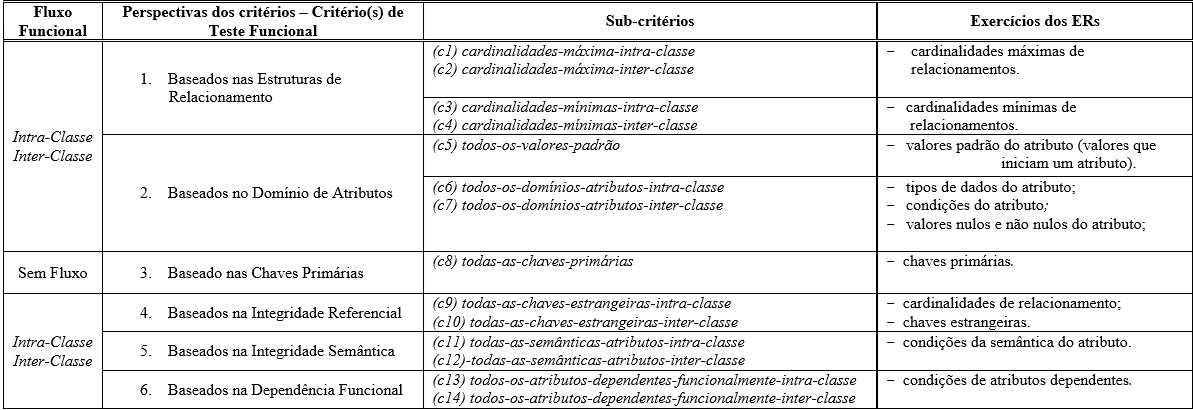
\includegraphics[width=0.9\textwidth]{./fig/figura4}
	\caption{Tabela das perspectivas dos crit�rios de Souza (2008)\cite{Souza} em compara��o sobre os crit�rios propostos}
	\label{fig:figura4}
\end{figure}


\section{T�cnica de Teste Mutante em Banco de Dados}
\label{sec:testeMutanteBd}